% PREAMBLE
% ***************************************************************************************************

\documentclass[smallheadings,headsepline,11pt,oneside,a4paper]{scrbook}

% Hier gibt man an, welche Art von Dokument man schreiben möchte.
% Possibilities in {}: scrartcl, scrreprt, scrbook, but also: article, report, book

\usepackage[english]{babel}		% changed to remove German
\usepackage[utf8]{inputenc}		% teilt LaTeX die Texcodierung mit. Bei Windowssystemen: ansinew
\usepackage[T1]{fontenc}		% ermöglicht die Silbentrennung von Wörtern mit Umlauten

\usepackage[usenames,dvipsnames]{color}

% PDF wird mit Lesezeichen (verlinktes Inhaltsverzeichnis) versehen (bei Betrachtung mit Acrobat Reader sichtbar)
\definecolor{farbelink}{rgb}{0,0,0}	% Definition der Linkfarbe für das PDF-File
\usepackage[pdftex,colorlinks=true,urlcolor=farbelink,linkcolor=farbelink,citecolor=farbelink]{hyperref}

\usepackage{lscape}

\usepackage{amssymb,amsmath}
\newcommand*\diff{\mathop{}\!\mathrm{d}}				% For nice differentials in integrals

\usepackage{geometry} 
\geometry{a4paper} 
\usepackage[parfill]{parskip}						% Activate to begin paragraphs with an empty line
\usepackage[pdftex]{graphicx}
\usepackage{epstopdf}
\DeclareGraphicsRule{.tif}{png}{.png}{`convert #1 `dirname #1`/`basename #1 .tif`.png}
\usepackage[margin=10pt,font=small,labelfont=bf]{caption}	% Package for picture captions

\usepackage[usenames]{color}

\usepackage{listings}							% Einfügen von Programmcode
\lstset{numbers=left, numberstyle=\tiny, numbersep=5pt}		% mit Zeilennummerierung links
\lstset{language=[77]Fortran}						% Programming language: Fortran77


%text with 2.5cm on both sides (A4=210mm)
\setlength{\textwidth}{160mm}
\setlength{\evensidemargin}{0in}
\setlength{\oddsidemargin}{0in}
\setlength{\columnsep}{0.25in}
%
%text with 2.5cm on top and 2.5cm on bottom (A4=297mm)
\setlength{\textheight}{247mm}
\setlength{\topmargin}{0pt}
\setlength{\headsep}{25pt}
\setlength{\headheight}{0pt}


%\typearea{12} % Increase the width of the printed areas (functions only in \documentclass with: scrreprt, scrartcl, scrbook)

\clubpenalty = 10000		% schliesst Schusterjungen aus
\widowpenalty = 10000		% schliesst Hurenkinder aus


\usepackage{fancyhdr}
\pagestyle{fancy}			% Selbst gestaltete Kopf-/Fusszeilen

%%% Fancy Header %%%%%%%%%%%%%%%%%%%%%%%%%%%%%%%%%%%%%%%%%%%%%%%%%%%%%%%%%%%%%%%%%%
% Fancy Header Style Options
\fancyhf{}
\fancyfoot{} 

\renewcommand{\chaptermark}[1]{				% Lower Case Chapter marker style
\markboth{\chaptername\ \thechapter.\ #1}{}}		%
\renewcommand{\sectionmark}[1]{				% Lower case Section marker style
\markright{\thesection.\ #1}}					%
\fancyfoot[R]{\thepage}						% Page number in the right on every page
\fancyhead[L]{\leftmark}						% Chapter in the right on even pages	
\fancyhead[L]{\rightmark}						% Section in the left on odd pages
\renewcommand{\headrulewidth}{0.3pt}			% Width of head rule

\fancypagestyle{plain}{						%
\fancyhf{}								% clear all header and footer fields
\fancyfoot[R]{\thepage}						% Page number in the right on every page
\fancyhead[L]{\leftmark}						% Chapter in the right on even pages
\renewcommand{\headrulewidth}{0.3pt}}			% Width of head rule


\setlength{\textheight}{21cm}					% Increase the height of the printed areas


\begin{document}

\frontmatter								% Roman numeral page numbers

% TITLE PAGE
% ***************************************************************************************************
% use FS or HS to identify the semester, FS (Fruehling) for spring semester, HS (Herbst) for fall semester

\begin{titlepage}
\begin{center}
    \vspace*{1cm}
    {\huge \bfseries  Development of a regularization term in a TLES code in OpenFOAM\\ }
    \vspace{2cm}
    {\large 
	Samuel Maloney\\
	~\\
	Computational Science and Engineering Master\\
	\vspace{3.5cm}
	Seminar in Fluid Dynamics for CSE HS 2017\\
	~\\
	Institute of Fluid Dynamics\\
	ETH Zürich\\
    }

\vspace{\stretch{1}}



{\large
	Supervisor: Daniel Oberle\\[\baselineskip]
	Professor: Patrick Jenny
}
\end{center}

\vspace*{2cm} % a bit of space at the bottom of the page

\end{titlepage}

%\clearpage\null


% Insert a blank page after the title page
\begin{titlepage}
\thispagestyle{empty}
\newpage
\mbox{}
\end{titlepage}


% ABSTRACT
% ***************************************************************************************************
% ABSTRACT
% ***************************************************************************************************
% with horizontal line
\begin{tabular}{p{0.9\textwidth}}
\chapter*{Abstract}

Temporal large eddy simulation (TLES) is a promising method to reduce computational costs compared to direct numerical simulation for turbulent flows while maintaining a high degree of accuracy, and offers several potential advantages over conventional spatial LES. A TLES method termed the temporal exact deconvolution model has previously been developed and then implemented in OpenFAOM but found to be unstable for large filter widths. In this project, a regularization term was designed, implemented, and tested to investigate its potential for stabilization of the method. Concurrently, a divergence cleaning method using the projection scheme was also added to the solver to test if non-zero divergence might be a source of the instabilities. Demonstration of the base method and the new stabilization strategies was realized using the Pitz-Daily backwards-facing step geometry provided in OpenFOAM, and a variety of different parameter combinations and model configurations were analyzed for both stability and for deviation from a stable baseline simulation. It was found that divergence cleaning improved the stability of the method only slightly, while the regularization term was able to stabilize every configuration tested if the strength of the regularization was made sufficiently high, although this stabilization came at the cost of substantial slowdown in the time-evolution of the flows towards their statistically stationary final states.

\end{tabular}




% TABLE OF CONTENTS
% ***************************************************************************************************

\tableofcontents
% This command inserts the table of contents. To ensure the page numbers are correct, the document should be generated twice!



% MAIN SECTION
% ***************************************************************************************************
% Folgende Befehle stehen für die Gliederung zur Verfügung: \chapter \section \subsection \subsubsection \paragraph
% Für Anführungszeichen: "` (CH-Tastatur: ZUERST: Shift-Tast und Taste 2, DANN: Shift-Taste und Taste ^)
% Für Schlusszeichen: "' (CH- Tastatur: ZUERST: Shift-Tast und Taste 2, DANN:  '-Taste, rechts neben der Null)
% For new paragraphs: leave a blank line.


\mainmatter	% Arabic page numbers


% 1. Introduction
%------------------------------------------------------------------------------------------------------------------------------
\chapter{Introduction}

%Chapter giving an introduction to the topic and the present work

DNS is computationally expensive, so go TLES!

An brief overview of some of the basic theory underpinning TLES is presented next, adapting from the work presented by Pruett \cite{Pruett2008} and Jenny \cite{Jenny2016}.

\section{TLES}

Since for TLES filtering is done during the course of the numerical experiments, the filtering operation must be \emph{causal}, ie. it must depend only upon the current and previous values of the quantity being filtered and not on any future values. Letting an overbar denote a time-filtered quantity and $T$ denote the characteristic filter width, one obtains the following causal time-filtering operation for some filter kernal $G(t,T)$:
\begin{equation}
\bar{f}(t,T)=\int_{-\infty}^{t}G(\tau -t;T)f(\tau)d\tau
\end{equation}

In this work only the exponential filter is discussed, namely:
\begin{equation}
G(t;T)=\frac{\exp(t/T)}{T} \longrightarrow \bar{f}(t,T)=\frac{1}{T}\int_{-\infty}^{t}\exp\left(\frac{\tau-t}{T}\right)f(\tau)d\tau
\end{equation}

which is a second order low-pass filter and has the transfer function:
\begin{equation}
H(\omega,T)=\frac{1}{1+iT\omega}
\end{equation}

Since the integral formulation would require storage of the quanitity at all previous time points in the simulation, the following equivalent differential form is used for implementation, as it can be integrated using standard time-marching schemes to update the filtered quantities at each step (where the explicit time-dependence of the quanitites is now dropped for convenience):
\begin{equation} \label{filter_diff}
\frac{\partial \bar{f}}{\partial t}=\frac{f-\bar{f}}{T}
\end{equation}

Applying such a filtering operation to the incompressible Navier-Stokes equations gives the following system for the evolution of temporally-filtered velocity fields, using the same initial condition as for the unfiltered fields $\bar{u}(0,x;T)=u(0,x)$:
\begin{equation}
\frac{\partial \bar{u}_j}{\partial x_j}=0
\end{equation}
\begin{equation} \label{TFNS}
\frac{\partial \bar{u}_i}{\partial t}+\frac{\partial (\bar{u}_i\bar{u}_j)}{\partial x_j}=-\frac{\partial \bar{p}}{\partial x_i}+\nu \frac{\partial^2 \bar{u}_i}{\partial x_j \partial x_j}-\frac{\partial \tau_{ij}}{\partial x_j}
\end{equation}

where $u$ is the fluid velocity, $p$ is the pressure, $\nu$ is the kinematic pressure, and subscripts $i,j\in\{1,2,3\}$ indicate the 3D cartesian direction. The element $\tau$ in the final term is referred to as the \emph{temporal stress tensor} and is defined as:
\begin{equation}
\tau_{ij}=\overline{u_i u}_j-\bar{u}_i\bar{u}_j
\end{equation}

Solving the temporally-filtered Navier-Stokes equations requires a residual-stress model to handle the unkown value $\overline{u_i u}_j$ and close the system. Stolz and Adams \cite{Stolz2001} dveloped an approximate deconvolution model (ADM) for for spatial LES which was then adapted for TLES by Pruett \cite{Pruett2008}. For this project, however, a new method termed the temporal exact deconvolution model TEDM created by Jenny \cite{Jenny2016} is used to provide the closure.

For the TEDM method, it is observed that by inserting the velocity field into the differential form of the filter given in Eq. (\ref{filter_diff}) the unfiltered field can be recovered as follows:
\begin{equation} \label{deconv}
u_i=\bar{u}_i+T\frac{\partial \bar{u}_i}{\partial t}
\end{equation}

The same Eq. (\ref{filter_diff}) can then be applied to the unknown quantity $\overline{u_i u}_j$ and the just obtained relation for the unfiltered field in Eq. (\ref{deconv}) can be inserted in the resulting expression to obtain the following:
\begin{equation}
\begin{split}
\frac{\partial{\overline{u_i u}_j}}{\partial t}&=\frac{u_i u_j-\overline{u_i u}_j}{T} \\
&=\frac{\left( \bar{u}_i+T\frac{\partial \bar{u}_i}{\partial t} \right) \left( \bar{u}_j+T\frac{\partial \bar{u}_j}{\partial t} \right)-\overline{u_i u}_j}{T} \\
&=\frac{\bar{u}_i \bar{u}_j-\overline{u_i u}_j}{T}+\bar{u}_i\frac{\partial \bar{u}_j}{\partial t}+\bar{u}_j\frac{\partial \bar{u}_i}{\partial t}+T\frac{\partial \bar{u}_i}{\partial t}\frac{\partial \bar{u}_j}{\partial t}
\end{split}
\end{equation}

This can then be rearranged to produce an equation for the time evolution of the temporal stress tensor $\tau$ containing only the known filtered velocities:
\begin{equation} \label{tau}
\frac{\partial \tau_{ij}}{\partial t}=-\frac{\tau_{ij}}{T}+T\frac{\partial \bar{u}_i}{\partial t}\frac{\partial \bar{u}_j}{\partial t}
\end{equation}

Suitable time integration schemes can then be used to solve Eqs. (\ref{TFNS}) and (\ref{tau}) in alternation to evolve the system in time.

\section{Regularization}

A regularization term based on work by \AA kervik et al. \cite{Akervik2006} was investigated as a potential means to improve the stability of the method, and is outlined here.

\section{Divergence Cleaning}

An implicit condition of the incompressible Navier-Stokes equations is that the divergence of the velocity field must be zero. However, numerical discretization schemes generally lead to non-zero values of the divergence which can be a potential source of isntability during simulations. To this end, explicit divergence cleaning (DC) using the projection scheme, following the procedure outlined in section 5 of the work by T\'oth \cite{Toth2000} for DC of magnetic fields, was also considered for possible stabilizing effects.

% 2. Implementation
%------------------------------------------------------------------------------------------------------------------------------
\chapter{Implementation}

% Chapter giving an overview of the implementation of the method in OpenFOAM

For this project, all implementation of the regularization term and divergence cleaning scheme was carried out in C++ using the open source OpenFOAM CFD code. A solver developed during a previous project at the institute, which implemented the fundamental TLES methodology, was used as a starting code. This solver already contained the necessary code for discretizing and solving Eq. (\ref{TFNS}) in the TFNS system for the filtered velocity, Eq. (\ref{tau}) for the temporal stress tensor, as well as computing the deconvoluted velocity field according to the TEDM and the mean filtered velocity field for statistical comparison and validation of the methods.

% 3. Results
%------------------------------------------------------------------------------------------------------------------------------
\chapter{Results}

% Chapter giving an overview of the numerical results obtained from the implementation

All simulations were carried out on the standard Pitz-Daily backward facing step geometry provided with OpenFOAM. The kinematic viscosity of $\nu=10^{-5}\,\mathrm{m}^2/\mathrm{s}$ and the inlet velocity of $u=10\,\mathrm{m}/\mathrm{s}$ were kept constant for all runs. Using this inlet velocity and the channel width $L=50.8\,\mathrm{mm}$, the Reynolds number of the flow can be approximated as: $$ Re=\frac{uL}{\nu}=50800$$

In order to provide a somewhat objective measure of comparison between the results of the method using different sets of parameters, a vertical line profile of the mean magnitude of the unfiltered velocity field was taken at the location shown in Fig. \ref{fig:line_location} after each run. As well, a simulation using a simple direct solution of the Navier-Stokes equations was performed as a baseline. It must be noted that this is not a true DNS comparison, as the simulation was performed on the same grid as used for all of the following TLES testing, and so is not fine enough to resolve the full range of scales of the system in general. Since such a fully-resolved DNS simulation was prohibitively time-consuming for this project, the under-resolved baseline case was considered acceptable to at least check for any large deviations resulting from the methods being tested, and for simplicity is referred to as DNS in the following analysis. The location of the line was chosen to be at the minimum value of the recirculation vortex in the DNS baseline, so as to have a distinct feature to compare with between runs.

\begin{figure}[!b]
\centering
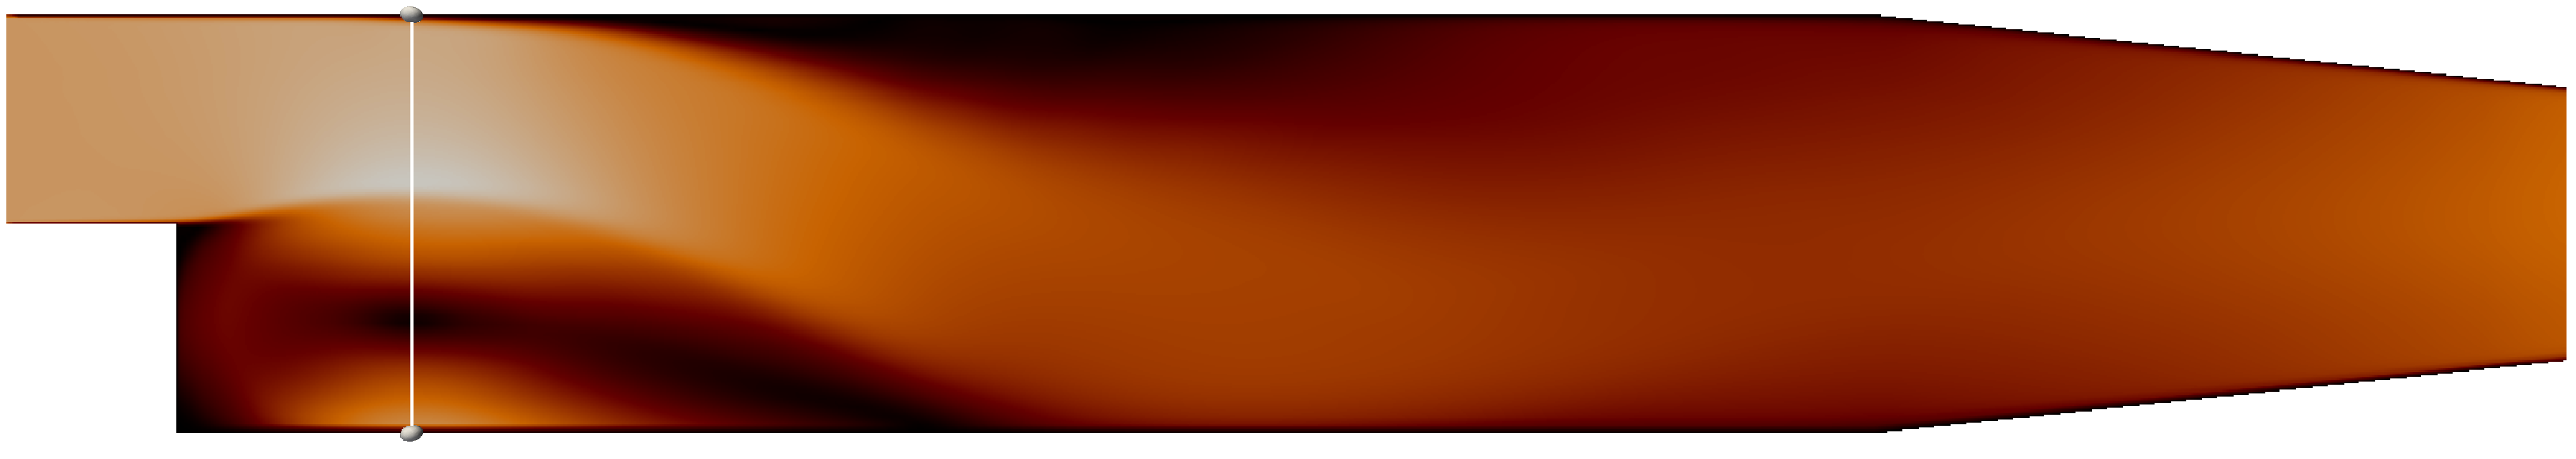
\includegraphics[width=0.75\textwidth]{figures/line_location.pdf}
\caption{Representative image of a $|\bar{u}|_{\mathrm{mean}}$ velocity field with a white line showing the location $x=28.6\,\mathrm{mm}$ past the step at which the comparison profiles were captured}
\label{fig:line_location}
\end{figure}

To start with, several simulations were run using only the basic TLES implementation, with no regularization or DC. This gave one free parameter to be varied, the filter width ratio $r$, and the resulting profiles were taken at an end time of $t_\mathrm{final}=0.1$ using a time step of $\Delta t=10^{-6}$ for all runs. It was observed that the simulation becomes unstable if the filter width is made too large, and so this time step was chosen as it gave a small range of values, up to $r\approx 28$, for which the base method was stable and any effects of varying $r$ in isolation could be observed.

The results of this initial study are shown in Fig. \ref{fig:line_data_no_reg} and the profiles from the various runs are seen to lie almost completely atop one another. This would seem to suggest that the effect of $r$ is minimal within the range of values which are stable without regularization.

\begin{figure}[!htb]
\centering
\includegraphics[width=0.75\textwidth]{figures/line_data_no_reg.pdf}
\caption{Comparison of line profiles from the $|\bar{u}|_{\mathrm{mean}}$ velocity field at $x=28.6\,\mathrm{mm}$ for various values of filter width $r$, taken at $t_\mathrm{final}=0.1$ using $\Delta t=10^{-6}$}
\label{fig:line_data_no_reg}
\end{figure}

The effects of adding DC to the method as per the projection method outlined in section \ref{sec:DC} were investigated next. A small increase in the stable range of the filter width $r$ was observed, with the largest stable value for $r$ increasing from $r=4.4$ to $r=4.7$ when $\Delta t=10^{-5}$, and from $r=28$ to $r=29$ for a $\Delta t=10^{-6}$ time step. Simulations were run with DC included in the simulations for the same already stable values of $r$ as in the previous set as well as for the now stabilized $r=29$ case, and the results are shown in Fig. \ref{fig:line_data_DC}. This allowed for potential comparison between the effects of DC both when it was and was not required to achieve stability in the first instance.

Unlike with the base TLES simulations, all of the runs with DC are seen to be no longer as perfectly concident with the baseline simulation, although the deviation is relatively minor and the variations of $r$ still appear to have little discernible impact on the results. Additionally, the runtime of the simulations increased by only between 5-11\% for the values of $r$ with a counterpart simulation not using DC, indicating decent efficiency of the DC implementation using an iterative solver with a relaxed tolerance, as discussed in sections \ref{sec:DC} and \ref{chap:Imp}.

\begin{figure}[!t]
\centering
\includegraphics[width=0.75\textwidth]{figures/line_data_DC.pdf}
\caption{Comparison of line profiles from the $|\bar{u}|_{\mathrm{mean}}$ velocity field at $x=28.6\,\mathrm{mm}$ for various values of filter width $r$ with divergence cleaning, taken at $t_\mathrm{final}=0.1$ using $\Delta t=10^{-6}$}
\label{fig:line_data_DC}
\end{figure}

\begin{figure}[!h]
\centering
\includegraphics[width=0.75\textwidth]{figures/line_data_reg.pdf}
\caption{Line profile from the $|\bar{u}|_{\mathrm{mean}}$ velocity field at $x=28.6\,\mathrm{mm}$ for $r=30$ with regularization. $\chi = 32000$, $\tilde{r}=100$, $t_\mathrm{final}=0.1$, and $\Delta t=10^{-6}$}
\label{fig:line_data_reg}
\end{figure}

In Fig. \ref{fig:line_data_reg} is shown the result of a run at $r=30$, using regularization with a control value of $\chi=32000$ to stabilize the simulation. This value of $\chi$ was chosen so as to be slightly larger than the minimal value for which the simulation was found to be stable for $r=30$, as discussed later in this chapter. It is observed that while the shape of the profile is very similar to the baseline case, the data shown was collected after propogating the simulation through 87X as many timesteps, to a $t_\mathrm{final}=8.4$ compared to $0.1$ for the baseline (and all other profiles shown.) The final time for comparison was chosen to be the time when the minimum of the recirculation vortex in the regularized run reached the same location as in the compared against baseline profile. Such good agreement between the profiles when matching such a recognizable feature as the vortex minimum suggests that the regularization stabilized simulation seems to evolve through the same sequence as without regularization, only at a \emph{much} slower rate.

Since most cases of instability in the simulation manifested within the first few dozen time steps (approx. 30-40 or less), and given the large number of parameter sets that needed to be tested, for the purposes of the following section a simulation was considered `stable' if it ran for 100 timesteps without failing. It is noted that a small number of the runs performed crashed even after 80+ timesteps, so this 100 timestep rule is certainly not an ironclad guarantee of stability over a much longer run. However, as in all of these cases it was the transition from stable to unstable that was under investigation, it suffices to warn that the reported minimal $\chi$ values required for stability should be regarded as providing only marginal stability, and slightly larger values might be safer in a real simulations to provide some margin of safety.

\begin{figure}[!tb]
\centering
\includegraphics[width=0.75\textwidth]{figures/min_chi_dt5_r100.pdf}
\caption{Minimum $\chi$ values required to stabilize simulation for various values of $r$, using $\Delta t=10^{-5}$ and $\tilde{r}=100$, and showing the linear least squares line regression}
\label{fig:min_chi_dt5_r100}
\end{figure}

\begin{figure}[!tb]
\centering
\includegraphics[width=0.75\textwidth]{figures/min_chi_dt5_r10.pdf}
\caption{Minimum $\chi$ values required to stabilize simulation for various values of $r$, using $\Delta t=10^{-5}$ and $\tilde{r}=10$, and showing the linear least squares line regression}
\label{fig:min_chi_dt5_r10}
\end{figure}

\begin{figure}[!tb]
\centering
\includegraphics[width=0.75\textwidth]{figures/min_chi_dt6_r100.pdf}
\caption{Minimum $\chi$ values required to stabilize simulation for various values of $r$, using $\Delta t=10^{-6}$ and $\tilde{r}=100$, and showing the linear least squares line regression}
\label{fig:min_chi_dt6_r100}
\end{figure}


% 4. Conclusion
%------------------------------------------------------------------------------------------------------------------------------
\chapter{Conclusion}

% Chapter giving an overview of the conclusions which can be drawn from the project

A stabilizing regularization term and divergence cleaning via the projection method have been implemented and integrated into a previously implemented temporally filtered large-eddy simulation (TLES) solver in OpenFOAM. The stability and output of the base method under different model parameters was studied and used as comparison against tests performed using the newly coded features to determine any stabilizing or other effects on the performance of the method.

Divergence cleaning was able to be efficiently implemented using an iterative solver with a relaxed tolerance, and was found to provide a measurable but small increase in the stable range of the filter width, along with very minor changes in the shape of its velocity line profile. The increase in stability seems to indicate that some non-zero divergence is present in the fields of the base method, but also that this was not the root cause of the instability, or at least not the sole root cause.

Regularization using the addition of a linear forcing term to the filtered Navier-Stokes momentum equation was found to be quite effective at stabilizing the solution. Any value of the filter width tested was able to be simulated successfully by setting the control parameter $\chi$ of the regularization sufficiently large. The evolution of the system towards a steady state was found to be greatly slowed by the regularization, but did produce a very similar velocity line profile when a recognizable feature was propagated to the same location in the geometry as in the non-regularized runs. A simulation using a time step for which no filter width was stable in the base method was also able to be stabilized by the regularization, and it was additionally found that starting the simulation with already time-evolved initial data allowed for successful simulation with some parameters that were unstable for uniform initial conditions. These two results, while needing additional investigation, suggest possibilities for mitigating the slow system evolution, either by using a larger time step, or by starting a simulation with a number of iterations using a stable parameter set in order to produce a more stable starting point for the full simulation using the desired, but potentially unstable, configuration of the method.


% Bibliography
%------------------------------------------------------------------------------------------------------------------------------
% Bibliography
%*****************************************************************************************************

% Bewtween \begin{thebibliography}{99} and \end{thebibliography} kann das Literaturverzeichnis erweitert werden. 
% The text in the braces directly after \bibitem can be used for citation with the \cite command.


\begin{thebibliography}{99}
\addcontentsline{toc}{chapter}{Bibliography}

\bibitem{Pruett2008} \textsc {C. Pruett,}  ``Temporal large-eddy simulation: theory and implementation,'' Theor. Comput. Fluid Dyn. \textbf{22}, 275 (2008).

\bibitem{Stolz2001} \textsc {S. Stolz, N.A. Adams, and L. Kleiser,}  ``An approximate deconvolution model for large-eddy simulation with application to incompressible wall-bounded flows,'' Phys. Fluids  \textbf{13}, 997 (2001).

\bibitem{Akervik2006} \textsc {A. \AA kervik, L Brandt, D. S. Henningson, J. H\oe pffner, O. Marxen, and P. Schlatter,}  ``Steady solutions of the Navier-Stokes equations by selective frequency damping,'' Phys. Fluids  \textbf{18}, 068102 (2006).

\bibitem{Jenny2016} \textsc {P. Jenny,}  ``Unsteady RANS closure,'' Unpublished (2016).

\bibitem{Toth2000} \textsc {G. T\'oth,}  ``The $\nabla \cdot B=0$ Constraint in Shock-Capturing Magnetohydrodynamics Codes,'' J. Comput. Fluids \textbf{161}, 605 (2000).

% Citation format for a book
%\bibitem{citation_reference} \textsc {Author,}  \emph{Book Title}, year, Publisher.
 
\end{thebibliography}


% Attachment
%------------------------------------------------------------------------------------------------------------------------------

%\appendix
%\renewcommand{\chaptermark}[1]{         		% Use "Attachment" instead of "Chapter" in in the header
%\markboth{Attachment\ \thechapter.\ #1}{}} 

%\include{Appendix}



% List of Figures
% ***************************************************************************************************
%\clearpage
%\phantomsection
%\addcontentsline{toc}{chapter}{List of Figures}
%\listoffigures

% List of Tables
% ***************************************************************************************************
%\clearpage
%\phantomsection
%\addcontentsline{toc}{chapter}{List of Tables}
%\listoftables


\end{document}
